
\documentclass[11pt]{article}

\newif\ifneuripsstyle
\IfFileExists{neurips_2025.sty}{%
  \neuripsstyletrue
  \usepackage[preprint]{neurips_2025}
}{%
  \neuripsstylefalse
  \usepackage[margin=1in]{geometry}
  \usepackage[numbers]{natbib}
}

\usepackage[utf8]{inputenc}
\usepackage[T1]{fontenc}
\usepackage{amsmath,amssymb,amsthm}
\usepackage{booktabs}
\usepackage{array}
\usepackage{tabularx}
\usepackage{graphicx}
\usepackage{xcolor}
\usepackage{hyperref}
\usepackage{microtype}
\usepackage{enumitem}
\usepackage{float}
\usepackage{algorithm}
\usepackage{algorithmic}
\usepackage{tikz}
\usepackage{pgfplots}
\pgfplotsset{compat=1.18}
\usetikzlibrary{arrows.meta,positioning,calc}

\hypersetup{
  colorlinks=true,
  linkcolor=blue!55!black,
  citecolor=blue!55!black,
  urlcolor=blue!55!black
}

\ifneuripsstyle\else
\setlength{\parindent}{0pt}
\setlength{\parskip}{5pt}
\fi

\newtheorem{definition}{Definition}
\newtheorem{remark}{Remark}

\newcommand{\TSP}{\textsc{TSP}}
\newcommand{\CVRP}{\textsc{CVRP}}
\newcommand{\VRP}{\textsc{VRP}}
\newcommand{\NCO}{\textsc{NCO}}
\newcommand{\AR}{\textsc{AR}}
\newcommand{\RRC}{\textsc{RRC}}
\newcommand{\PRC}{\textsc{PRC}}
\newcommand{\LEHD}{\textsc{LEHD}}
\newcommand{\SIL}{\textsc{SIL}}
\newcommand{\BTP}{\textsc{BTP}}
\newcommand{\method}{\textsc{STAR}}
\newcommand{\EAM}{\textsc{EAM}}
\newcommand{\cA}{\mathcal{A}}
\newcommand{\cE}{\mathcal{E}}
\newcommand{\cN}{\mathcal{N}}
\newcommand{\cY}{\mathcal{Y}}
\newcommand{\cost}{C}
\newcommand{\gap}{\operatorname{gap}}
\newcommand{\clip}{\operatorname{clip}}
\newcommand{\argmin}{\operatorname*{arg\,min}}
\newcolumntype{Y}{>{\centering\arraybackslash}X}
\newcolumntype{L}{>{\raggedright\arraybackslash}X}

\title{\method{}: Bounded Transition Inference for Neural Routing}

\author{Anonymous Authors\\
Anonymous Institution\\
\texttt{anonymous@example.com}}
\date{}

\begin{document}
\maketitle

\begin{abstract}
Autoregressive neural routing policies are trained to make local next-node decisions, but standard test-time inference often asks them to construct a full long trajectory or reconstruct a broad coupled segment. This creates an inference-granularity mismatch: the model may remain locally useful, while the inference procedure creates long horizons, compounding state drift, and sparse feedback. We introduce \method{}, a training-free test-time adaptation framework that changes the inference granularity to bounded route-conditioned transitions. \method{} repeatedly queries a fixed policy on local masked states, projects each proposed transition back to a feasible trajectory with local trajectory projection (\BTP{}), and stores positive introduced-edge feedback in episodic memory (\EAM{}) to shape future logits on the same instance. Thus extra inference compute becomes stateful guidance without gradient updates or weight changes. On benchmark routing instances, \method{} obtains valid solution coverage across the evaluated groups, gives competitive gap-time behavior, and improves substantially over autoregressive construction and reconstruction baselines on constrained routing. The results support inference-interface design as a complementary axis to architecture and training for zero-shot neural routing.
\end{abstract}

\section{Introduction}

Vehicle routing problems (VRPs) are central combinatorial optimization problems with broad applications in transportation, logistics, and supply-chain planning \citep{VRPAPP,nrs_survey}. Because routing variants are computationally hard, practical solvers rely on exact methods, local search, and highly engineered heuristics to obtain high-quality solutions within acceptable time budgets \citep{lkhtsp,lkhcvrp,hgs}. These solvers are powerful, but their performance depends on carefully designed search components, neighborhoods, candidate sets, and parameter choices.

Neural combinatorial optimization (NCO) aims to reduce this manual design burden by learning heuristic decisions from data \citep{l2osurvey,MLCO}. In routing, constructive autoregressive policies are especially common: a neural model scores the next feasible node conditioned on the instance, partial route, current node, and feasibility mask. Pointer Networks and attention-based models established this decoding view \citep{pointernetwork,attentionmodel}; later work improved training diversity, model structure, and large-scale behavior through multi-start policies, quotient-state formulations, decoder-heavy architectures, and self-improved learning \citep{pomo,bq,lehd,sil}. Once trained, these policies can generate solutions quickly, making them attractive as reusable learned routing components.

However, zero-shot generalization remains a central weakness of neural routing solvers. Models trained on small synthetic instances often degrade on larger or more structured benchmark instances, and recent surveys argue that conventional synthetic evaluation can overstate generalization performance \citep{nrs_survey}. One response is to train stronger or larger-scale models, but this raises label, rollout, and search-space costs. Another line keeps the learned model fixed and changes the test-time procedure through decomposition, local policies, reconstruction, or projection \citep{learn2delegate,htsp,glop,invit,ttpl}. These methods share an important premise: useful local decision structure can remain available even when direct full-instance deployment fails.

This paper studies a complementary failure mode. Autoregressive routing policies fail not only because the test instances are larger, but because standard inference uses an unsuitable granularity. Full construction couples the neural query horizon to the global route length: as the instance grows, the model must make more sequential decisions before a complete solution is evaluated. Reconstruction shortens this horizon by conditioning on an existing route, but broad reconstruction can still change many route relations before receiving one scalar improvement signal \citep{lehd,sil}. In both cases, the learned next-node policy is used as a long-horizon or weak-credit generator, even though it was trained as a local conditional decision rule.

We introduce \method{}, a training-free inference interface that changes the inference granularity to bounded route-conditioned transitions. Each iteration performs a short local decode inside a reference trajectory, projects the proposal back to a feasible locally corrected trajectory through local trajectory projection (\BTP{}), and assigns positive introduced-edge credit through episodic memory (\EAM{}). The neural policy supplies learned local preferences, projection makes the proposed transition evaluable, and memory turns repeated test-time calls into stateful adaptation without gradient updates or weight changes.

We evaluate \method{} on the generalization-focused benchmark protocol of \citet{nrs_survey}. The empirical claim is not that \method{} replaces classical optimization, but that changing inference granularity improves the gap-time behavior of autoregressive neural routing. The method gives a competitive gap-time tradeoff on single-route benchmarks and stronger gains on capacitated routing, where capacity, depot structure, and route-boundary interactions make local validation especially important.

Our contributions are as follows:
\begin{enumerate}[leftmargin=*,noitemsep]
  \item We identify inference-granularity mismatch as a practical failure mode of autoregressive neural routing under length extrapolation: standard inference couples the neural query horizon and feedback granularity to the global instance size.
  \item We introduce \method{}, a training-free inference interface that queries a neural policy through bounded route-conditioned transitions, locally projects each proposal, and reuses positive introduced-edge feedback through bounded logit shaping.
  \item We provide diagnostics for bounded inference, including neural horizon, changed-edge intervention size, local credit density, proposal diversity, and gap-time scaling.
  \item We evaluate \method{} on representative routing benchmarks, showing improved gap-time behavior over construction and reconstruction baselines, with the clearest gains on constrained routing instances.
\end{enumerate}

\section{Related Work}

Existing neural routing methods can be viewed by the granularity of the decision or search step they ask a learned model to handle. This perspective is useful for our setting because \method{} does not propose a new neural architecture or training objective. Instead, it changes how an autoregressive model is queried during inference.

\subsection{Constructive Neural Routing}

Constructive NCO methods learn to generate routing solutions directly from the instance. Early work introduced sequence and attention-based decoders for selecting nodes autoregressively \citep{pointernetwork,attentionmodel}. Subsequent methods improve construction through better treatment of solution symmetries, more expressive state abstractions, heavier decoding modules, or self-improved training and inference \citep{pomo,bq,lehd,sil}. These advances strengthen the learned policy, but the common inference interface remains full-trajectory generation: the model is asked to keep selecting nodes until the complete route is formed. Under length extrapolation, this makes the neural query horizon grow with the instance size. \method{} is complementary to these models because it keeps the autoregressive action interface but changes the inference granularity from a complete trajectory to a bounded local transition.

\subsection{Reconstruction and Neural-Guided Improvement}

Another line of work uses learned models inside an improvement procedure rather than as a one-shot constructor. Reconstruction-based methods condition on an existing solution, remove part of it, and ask a decoder to rebuild the missing structure \citep{lehd,sil}. More general neural-guided improvement methods use learned heatmaps, scores, or candidate sets inside stronger search pipelines \citep{difusco,gfacs,neurolkh}. These approaches show that learned signals can be useful during test-time optimization, not only during initial construction. The difference is the intervention scale. Broad reconstruction and many improvement pipelines evaluate a large coupled modification before receiving feedback, so credit is attached to many changed route relations at once. \method{} uses a narrower intervention: a bounded route-conditioned transition whose effect is locally projected and credited to introduced relations.

\subsection{Decomposition, Local Policies, and Projection}

Large-scale generalization is also addressed by reducing the effective problem size or by changing the input distribution seen by the model. Decomposition methods divide a large instance into subproblems before applying a learned or classical solver, while local-policy methods restrict each decision to a candidate neighborhood \citep{learn2delegate,htsp,glop,invit}. These strategies reduce the action space, but they can also create local subgraphs whose distribution differs from the training instances. Projection-based test-time methods directly target this mismatch by transforming local candidate neighborhoods toward the distribution on which the model was trained \citep{ttpl}. \method{} addresses a different but compatible mismatch. Projection aligns the input geometry presented to a local decision rule; bounded transition inference aligns the horizon and feedback structure of the query made to that rule. Both views treat test-time inference as a design object rather than a fixed consequence of the trained model.

\section{Preliminaries}
\label{sec:prelim}

This section introduces the notation used to describe inference granularity. We first define the routing objective, then the autoregressive policy interface, and finally the reference-solution setting used by reconstruction and by \method{}.

\paragraph{Routing objective.}
Let $x$ be a routing instance with node set $V$, feasible solution set $\cY(x)$, and benchmark distance $d_x(i,j)$ between nodes $i,j\in V$. A feasible solution $y\in\cY(x)$ induces route relations $E(y)$, represented as an edge set for single-route settings and as an edge multiset when multiple depot-rooted routes are present. The objective value is
\begin{equation}
  \cost_x(y)=\sum_{(i,j)\in E(y)}d_x(i,j),
  \label{eq:cost}
\end{equation}
and the percentage optimality gap with respect to a reference cost $\cost_x^\star$ is
\begin{equation}
  \gap_x(y)=100\cdot\frac{\cost_x(y)-\cost_x^\star}{\cost_x^\star}.
  \label{eq:gap}
\end{equation}

\paragraph{Autoregressive routing policies.}
An autoregressive policy with parameters $\theta$ constructs a solution through a sequence of states $s_t$ and feasible actions $a_t\in\cA(x,s_t)$:
\begin{equation}
  P_\theta(y\mid x)=\prod_{t=1}^{T(x,y)}P_\theta(a_t\mid x,s_t),
  \label{eq:ar}
\end{equation}
where $T(x,y)$ is the number of decisions required to emit solution $y$. The state contains the partial route, current node, visited mask, and problem-specific feasibility variables such as remaining capacity. The policy logit for action $a$ is denoted by $\ell_\theta(a\mid x,s)$. Standard greedy decoding selects the feasible action with the largest logit at each step, while sampling-based decoding draws from the policy distribution and returns the best complete solution among multiple rollouts. In both cases, the neural query horizon is the number of sequential policy calls made before a proposal can be evaluated.

\paragraph{Reference-solution inference.}
Many inference-time procedures operate relative to a reference solution rather than constructing from an empty route. Given a reference trajectory $y$ and a proposal $\hat y$, the modified route relations are summarized by
\begin{equation}
  q(\hat y,y)=|E(\hat y)\triangle E(y)|.
  \label{eq:changed-relations}
\end{equation}
The scalar improvement is $\Delta C=\cost_x(y)-\cost_x(\hat y)$. Reconstruction-based inference uses this setting by removing a segment or subset of route decisions, asking the policy to rebuild the missing part under feasibility constraints, and evaluating the resulting complete proposal. This reference-solution view is also used by \method{}, but with a smaller intervention scope.

\section{Inference Granularity Mismatch}
\label{sec:bottleneck}

When solving large routing instances, the challenge is not only that the input distribution changes. The inference procedure also changes the granularity of work assigned to the neural policy. We use the term inference unit to denote the route structure assigned to one neural query before its outcome is evaluated. A model trained to score local next-node decisions may be queried as a long-horizon trajectory generator or as a broad reconstruction module. In this section, we isolate this mismatch because it motivates the design of \method{}.

\paragraph{Full construction asks for a long trajectory.}
Greedy decoding and independent sampling use the policy as a full-trajectory generator. Under scale shift, $T(x,y)$ grows with the instance and route length, so each additional neural decision can push later states away from the distribution induced by training rollouts. Repeating independent rollouts increases coverage, but it leaves the inference granularity unchanged: the policy is still responsible for an entire trajectory.

\paragraph{Broad reconstruction asks for a coupled segment.}
Reconstruction conditions on a reference trajectory and asks the policy to complete a missing part. This is more structured than one-shot construction, but the feedback can still be attached to a broad intervention. Using the changed-relation count in Eq.~\eqref{eq:changed-relations}, a scalar improvement provides average proposal-level credit
\begin{equation}
  \rho(\hat y;y)=\frac{\Delta C}{\max(1,q(\hat y,y))}.
  \label{eq:credit-density}
\end{equation}
As $q$ grows, the same outcome becomes a weaker signal about which neural decisions were useful.

\paragraph{A useful granularity should be local and feedback-carrying.}
The desired inference unit should keep the neural horizon bounded, preserve the construction-compatible action interface, and attach feedback to a small set of introduced route relations. This does not require changing the learned model. It requires changing the way inference queries the model and reuses the outcomes of those queries. \method{} instantiates this principle with bounded route-conditioned transitions.

\section{\method{}: Bounded Transition Inference}
\label{sec:method}

\subsection{Framework}

\method{} keeps the neural routing model fixed and changes only the inference loop. It maintains a reference trajectory $y_t$, a best-so-far trajectory $y_t^\star$, and an episodic introduced-edge memory $M_t:\cE\rightarrow[-M_{\max},M_{\max}]$ over route relations. Each iteration uses the bounded transition granularity from Section~\ref{sec:bottleneck}: select route-conditioned states, decode short transition sequences, project each proposal locally, and credit introduced edges that improve the reference.

The framework has three parts: bounded local decoding, local trajectory projection, and episodic introduced-edge memory. The neural model provides learned local preferences. \BTP{} makes the bounded transition feasible and locally sharp enough to evaluate. \EAM{} reuses positive local evidence by biasing future policy calls on the same instance. This is stateful test-time adaptation, but not weight adaptation: memory can be initialized, clipped, cleared, or inspected without changing $\theta$.

\begin{figure}[t]
\centering
\small
\fbox{
\begin{minipage}{0.94\linewidth}
\begin{tabularx}{\linewidth}{>{\raggedright\arraybackslash}X c >{\raggedright\arraybackslash}X}
\textbf{Full construction or broad reconstruction} &&
\textbf{\method{} bounded transition inference} \\
\midrule
A full trajectory or large segment is decoded from the policy. &&
A bounded transition is decoded inside a reference trajectory. \\
Search feedback is observed only after many coupled decisions. &&
Feedback is assigned to introduced route relations with positive local advantage. \\
Post-hoc correction after every proposal is expensive because many edges may change. &&
Local projection is restricted to endpoints and candidate neighbors affected by the transition. \\
Repeated calls do not create instance-specific preferences inside the neural policy. &&
An episodic prior biases future masked decoding calls on the same instance. \\
\end{tabularx}
\end{minipage}
}
\caption{Conceptual comparison between conventional autoregressive inference and \method{}. The method preserves the autoregressive action interface while constraining each neural call to a local, projectable, feedback-carrying query.}
\label{fig:interface}
\end{figure}

\begin{algorithm}[t]
\caption{\method{} inference with a fixed autoregressive policy.}
\label{alg:star}
\small
\begin{algorithmic}[1]
\REQUIRE Instance $x$, autoregressive policy $P_\theta$, initial solution $y_0$, budget $B$, transition budget $r$, candidate width $K$, proposals $S$
\STATE Initialize reference trajectory $y \leftarrow y_0$, best trajectory $y^\star \leftarrow y_0$, and memory $M(e)\leftarrow 0$
\STATE Build candidate lists $\cN_K(i)$
\FOR{$t=1,\ldots,B$}
    \STATE Select route-conditioned states and candidate masks for $S$ bounded transitions
    \STATE Decode transition sequences under the shaped distribution in Eq.~\eqref{eq:shaped}
    \STATE Apply each transition to the reference trajectory and project it with \BTP{}
    \STATE Let $\hat y_t$ be the best projected candidate
    \STATE Update $M$ from proposals with positive local advantage over $y$
    \STATE $y\leftarrow \hat y_t$
    \IF{$\cost_x(y)<\cost_x(y^\star)$}
        \STATE $y^\star\leftarrow y$
    \ENDIF
\ENDFOR
\STATE \textbf{return} $y^\star$
\end{algorithmic}
\end{algorithm}

\subsection{Route-Conditioned Local Decoding}

At iteration $t$, let $u_t$ be the current route anchor and let $C_t\subseteq V$ be the feasible candidate set exposed to the decoder. The local state is
\begin{equation}
  s^{\mathrm{local}}_0=(x,\ y_t,\ u_t,\ C_t,\ \text{mask},\ \text{feasibility state}).
  \label{eq:local-state}
\end{equation}
The decoder selects a short sequence $\sigma_t=(a_1,\ldots,a_m)$, with $m$ controlled by a transition budget $r$. Each selected action updates the local route-conditioned state and introduces a short chain of new route relations,
\begin{equation}
  (u_t,a_1),(a_1,a_2),\ldots,(a_{m-1},a_m),
  \label{eq:splice}
\end{equation}
while the rest of the reference trajectory supplies the surrounding context before projection.

The state in Eq.~\eqref{eq:local-state} is a restricted construction state. The route context, current anchor, visited mask, and feasible-action mask are represented in the same form as ordinary autoregressive decoding, while the reference trajectory supplies global context. The model therefore selects plausible transitions within a small feasible set under its learned sequential structure. By construction, every local decode has a bounded horizon, independent of the global instance size.

For unconstrained routing, this corresponds to a local autoregressive transition over customer order. For capacitated routing, the same principle is applied with route-boundary information and remaining capacity in the local mask, so the transition can be evaluated by capacity-preserving projection.

\begin{figure}[t]
\centering
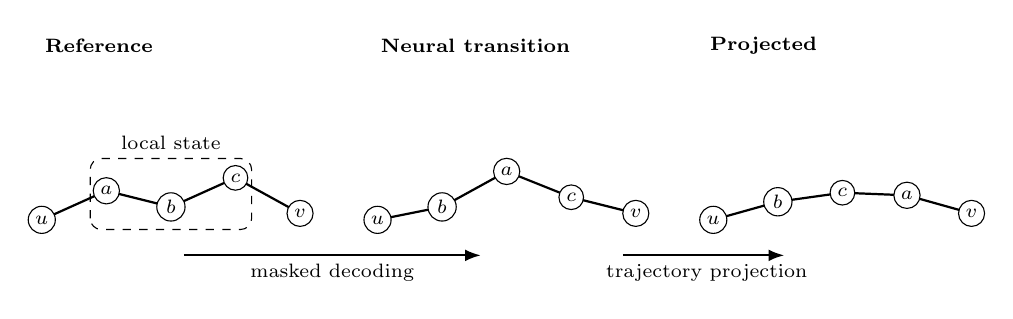
\begin{tikzpicture}[scale=0.82, every node/.style={font=\scriptsize}]
\node[anchor=west] at (-0.1,2.7) {\textbf{Reference}};
\draw[thick] (0,0) -- (1.0,0.45) -- (2.0,0.2) -- (3.0,0.65) -- (4.0,0.1);
\foreach \x/\y/\name in {0/0/$u$,1.0/0.45/$a$,2.0/0.2/$b$,3.0/0.65/$c$,4.0/0.1/$v$}
  \node[circle,draw,fill=white,inner sep=1.5pt] at (\x,\y) {\name};
\draw[rounded corners,dashed] (0.75,-0.15) rectangle (3.25,0.95);
\node at (2.0,1.2) {local state};

\node[anchor=west] at (5.1,2.7) {\textbf{Neural transition}};
\draw[thick] (5.2,0) -- (6.2,0.2) -- (7.2,0.75) -- (8.2,0.35) -- (9.2,0.1);
\foreach \x/\y/\name in {5.2/0/$u$,6.2/0.2/$b$,7.2/0.75/$a$,8.2/0.35/$c$,9.2/0.1/$v$}
  \node[circle,draw,fill=white,inner sep=1.5pt] at (\x,\y) {\name};
\draw[-{Latex[length=2mm]},thick] (2.2,-0.55) -- (6.8,-0.55);
\node at (4.5,-0.82) {masked decoding};

\node[anchor=west] at (10.2,2.7) {\textbf{Projected}};
\draw[thick] (10.4,0) -- (11.4,0.28) -- (12.4,0.42) -- (13.4,0.38) -- (14.4,0.1);
\foreach \x/\y/\name in {10.4/0/$u$,11.4/0.28/$b$,12.4/0.42/$c$,13.4/0.38/$a$,14.4/0.1/$v$}
  \node[circle,draw,fill=white,inner sep=1.5pt] at (\x,\y) {\name};
\draw[-{Latex[length=2mm]},thick] (9.0,-0.55) -- (11.5,-0.55);
\node at (10.3,-0.82) {trajectory projection};
\end{tikzpicture}
\caption{Schematic illustration of a local transition. The autoregressive policy is queried for a bounded masked transition inside the reference trajectory, followed by \BTP{} around the changed edges.}
\label{fig:splice}
\end{figure}

\subsection{Projection Makes the Transition Evaluable}

Let $D_t$ and $I_t$ denote the deleted and inserted edges from a local transition. The affected endpoints are
\begin{equation}
  A_t^{\mathrm{end}}=\{i:\exists j,\ (i,j)\in D_t\cup I_t \text{ or } (j,i)\in D_t\cup I_t\}.
  \label{eq:endpoints}
\end{equation}
With candidate lists $\cN_K(i)$, \BTP{} defines the projection region
\begin{equation}
  \Omega_t=A_t^{\mathrm{end}}\cup\bigcup_{i\in A_t^{\mathrm{end}}}\cN_K(i).
  \label{eq:scope}
\end{equation}
For single-route instances, \BTP{} applies candidate-graph 2-opt segment reversals whose tested edges touch $\Omega_t$. For capacitated multi-route instances, it adds capacity-feasible inter-route relocate, swap, and 2-opt* tail-exchange moves. The role of projection is not to replace the neural proposal with an unconstrained solver. It is to preserve the relationship between a decoded local sequence and its locally corrected trajectory, so the bounded transition can be evaluated without damaging distant parts of the route.

\subsection{Episodic Introduced-Edge Memory Turns Calls into Adaptation}

Let $\phi(s,a)$ be the set of edges introduced when action $a$ is selected in state $s$. The memory score is
\begin{equation}
  G_t(s,a)=\frac{1}{\max(1,|\phi(s,a)|)}\sum_{e\in\phi(s,a)}M_t(e).
  \label{eq:memory-score}
\end{equation}
The dynamic logit-shaping distribution is defined as
\begin{equation}
  \widetilde P_t(a\mid x,s)=
  \frac{
  \exp((\ell_\theta(a\mid x,s)+\lambda G_t(s,a)-\beta\Delta c(s,a))/\tau)
  }{
  \sum_{b\in\cA(x,s)}
  \exp((\ell_\theta(b\mid x,s)+\lambda G_t(s,b)-\beta\Delta c(s,b))/\tau)
  }.
  \label{eq:shaped}
\end{equation}
Here $\lambda\ge0$ controls the strength of episodic memory, $\beta\ge0$ controls the distance feature, and $\tau>0$ denotes the sampling temperature. These values are fixed within a run unless explicitly varied in a sensitivity study. The feature $\Delta c(s,a)$ is a normalized one-step distance proxy. If $p_s$ denotes the current endpoint in the local transition, we compute
\begin{equation}
  \Delta c(s,a)=\frac{d_x(p_s,a)}{\bar d_x},
  \label{eq:insertion}
\end{equation}
where $\bar d_x$ is the mean distance over the local candidate list. This term is not a learned component; it is a test-time geometric prior that discourages obviously expensive transitions when the masked action set contains several plausible neural choices.

Given a reference trajectory $y_t$ and projected candidate $\hat y_t$, define
\begin{equation}
  A_t(\hat y_t;y_t)=
  \frac{\cost_x(y_t)-\cost_x(\hat y_t)}{\max(\cost_x(y_t),\epsilon)}
  \label{eq:advantage}
\end{equation}
where $\epsilon>0$ is a small numerical constant that prevents division by zero. Define the introduced edges as
\begin{equation}
  \Delta E_t^+=E(\hat y_t)\setminus E(y_t).
  \label{eq:introduced}
\end{equation}
\EAM{} updates episodic memory according to
\begin{equation}
  M_{t+1}(e)=
  \begin{cases}
  \clip(M_t(e)+\eta A_t(\hat y_t;y_t),-M_{\max},M_{\max}),
  & \text{if } A_t(\hat y_t;y_t)>0 \text{ and } e\in\Delta E_t^+,\\
  M_t(e), & \text{otherwise.}
  \end{cases}
  \label{eq:update}
\end{equation}
where $\eta>0$ is the memory step size.

The update is positive-only in the reported experiments. Non-improving proposals are not treated as negative evidence because an unsuccessful projected trajectory may arise from the selected state, the decoded sequence, the projection width, or the quality of the reference trajectory. In contrast, a proposal with positive advantage provides a cleaner credit signal. The clipping threshold prevents a small number of early improvements from dominating the neural logits throughout inference.

The memory score in Eq.~\eqref{eq:memory-score} is normalized by the number of introduced edges represented by the action. This avoids assigning larger scores to actions only because they touch more memory entries. Since every memory entry is clipped to $[-M_{\max},M_{\max}]$, the absolute memory-induced logit shift is bounded by $\lambda M_{\max}$. Thus, \EAM{} implements bounded, training-free inference guidance: it can shape the policy distribution without silently replacing learned logits unless $\lambda$ is deliberately set large.

\subsection{Reference Update and Properties}

The reported experiments use a best-proposal reference update with monotone best-so-far tracking:
\begin{equation}
  y_{t+1}=
  \argmin_{\hat y\in\widehat{\cY}_t}\cost_x(\hat y),
  \label{eq:accept}
\end{equation}
where $\widehat{\cY}_t$ is the set of projected proposals generated from reference trajectory $y_t$. The best-so-far solution is updated separately,
\begin{equation}
  y_{t+1}^\star=
  \begin{cases}
  y_{t+1}, & \cost_x(y_{t+1})<\cost_x(y_t^\star),\\
  y_t^\star, & \text{otherwise.}
  \end{cases}
  \label{eq:best}
\end{equation}
Thus the reference trajectory can move to a different projected proposal for exploration, while the returned solution remains monotone.

Several useful properties follow directly from the algorithm design. First, the local decoding horizon is bounded by the transition budget $r$. Second, episodic memory values remain bounded because every update is clipped to $[-M_{\max},M_{\max}]$. Third, for fixed outer budget $B$, proposal count $S$, and transition budget $r$, the method performs at most $BSr$ autoregressive action selections, apart from encoder reuse. Fourth, best-so-far tracking gives an anytime output even when the reference trajectory is allowed to move for exploration. These properties characterize the computational and guidance behavior of the inference loop.

\section{Experiments}
\label{sec:experiments}

The experiments test whether bounded transition inference addresses the inference-granularity mismatch. We organize the section around reviewer-facing questions: (1) does \method{} improve gap-time behavior on benchmark routing instances; (2) does additional inference compute remain useful when the neural horizon is bounded; (3) which parts of the bounded transition matter; (4) when does memory help; (5) how sensitive is the method to local scope; and (6) does the interface transfer across architectures?

We follow the generalization-focused evaluation pipeline of \citet{nrs_survey}. Rather than drawing fresh synthetic test sets, the pipeline evaluates on established benchmark and challenge instances with available best-known solutions and Euclidean distance conventions. The single-route benchmark pool combines TSPLIB \citep{tsplib}, National TSP, VLSI, and DIMACS challenge instances \citep{national_tsp,vlsi_tsp,dimacs_tsp}; the capacitated benchmark pool uses CVRPLIB \citep{cvrplib}. Results are grouped by node count into small $(0,1K)$, medium $[1K,10K)$, and large $[10K,100K]$ buckets, matching the survey protocol. We report the representative variants separately because they stress different aspects of inference granularity: long sequential horizons in the single-route setting and route-level capacity/depot interactions in capacitated routing.

Unless otherwise stated, experiments instantiate the neural logit provider with \SIL{} \citep{sil}. This choice gives a strong autoregressive decoder while keeping the study focused on the inference interface: \method{} does not retrain or update model weights. The primary metric is average optimality gap to the best-known solution, complemented by valid feasible coverage and runtime. Validation details and per-instance extremes are deferred to the appendix.

\subsection{Does Bounded Transition Inference Improve Gap-Time Behavior?}

\begin{table}[t]
\centering
\caption{Completed \method{} results on survey benchmark groups.}
\label{tab:star-results}
\small
\renewcommand{\arraystretch}{0.9}
\begin{tabularx}{\textwidth}{llYYYYYYYY}
\toprule
& & & & \multicolumn{4}{c}{Gap statistics} & \multicolumn{2}{c}{Runtime} \\
\cmidrule(lr){5-8} \cmidrule(lr){9-10}
Problem & Scale group & Instances & Valid & Avg & Median & Best & Worst & Avg & Total \\
\midrule
\TSP{} & $n<1K$ & 69 & 69/69 & 0.36\% & 0.10\% & 0.00\% & 3.21\% & 54.02s & 1.04h \\
\TSP{} & $1K\le n<10K$ & 109 & 109/109 & 3.42\% & 3.12\% & 0.62\% & 8.48\% & 1.43m & 2.60h \\
\midrule
\CVRP{} & $n<1K$ & 99 & 99/99 & 2.47\% & 2.45\% & 0.14\% & 5.73\% & 2.23m & 3.68h \\
\CVRP{} & $1K\le n<10K$ & 5 & 5/5 & 4.76\% & 4.74\% & 3.32\% & 6.44\% & 14.76m & 1.23h \\
\CVRP{} & $10K\le n\le100K$ & 6 & 6/6 & 7.64\% & 7.09\% & 5.74\% & 10.53\% & 44.21m & 4.42h \\
\bottomrule
\end{tabularx}
\end{table}

Table~\ref{tab:star-results} shows that \method{} returns valid feasible solutions across the evaluated benchmark groups. On the single-route benchmark, the method is not the strongest high-budget reconstruction procedure, but it gives a much faster route to competitive quality. On the capacitated benchmark, the advantage is sharper: local transition proposals are immediately validated against capacity and depot structure, and this bounded feedback granularity improves over the autoregressive construction and reconstruction baselines reported under the same pipeline. Appendix~\ref{app:large-comparison} gives the broader survey-shaped comparison, including larger-scale rows for other methods.

\subsection{Does Bounded Inference Use Extra Compute Effectively?}

We hypothesize that bounding the neural horizon mitigates OOD length extrapolation and allows additional test-time compute to remain useful over longer inference budgets. Figure~\ref{fig:scaling} supports this hypothesis. Standard sampling improves only early and then saturates, because independent rollouts repeatedly reflect the same learned distribution. Broad reconstruction improves further, but the larger query granularity makes each proposal expensive and weakens local credit assignment. In contrast, our approach produces a smoother improvement curve because each additional iteration creates local feedback that changes later proposals through \EAM{}.

\begin{figure}[t]
\centering
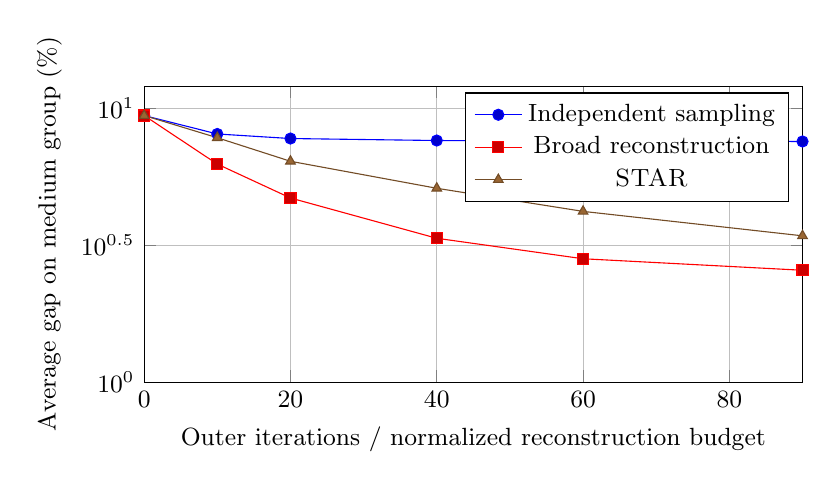
\begin{tikzpicture}
\begin{axis}[
    width=0.82\linewidth,
    height=0.44\linewidth,
    xlabel={Outer iterations / normalized reconstruction budget},
    ylabel={Average gap on medium group (\%)},
    ymode=log,
    xmin=0, xmax=90,
    ymin=1, ymax=12,
    grid=both,
    legend style={at={(0.98,0.98)},anchor=north east,font=\small},
    tick label style={font=\small},
    label style={font=\small}
]
\addplot+[mark=*] coordinates {(0,9.40) (10,8.05) (20,7.75) (40,7.62) (60,7.58) (90,7.56)};
\addlegendentry{Independent sampling}
\addplot+[mark=square*] coordinates {(0,9.40) (10,6.25) (20,4.70) (40,3.35) (60,2.82) (90,2.56)};
\addlegendentry{Broad reconstruction}
\addplot+[mark=triangle*] coordinates {(0,9.40) (10,7.80) (20,6.40) (40,5.10) (60,4.20) (90,3.42)};
\addlegendentry{\method{}}
\end{axis}
\end{tikzpicture}
\caption{Inference-scaling behavior on the medium group. The comparison reports iteration-level scaling rather than hardware-normalized runtime and measures solution-quality improvement as additional test-time iterations are allocated.}
\label{fig:scaling}
\end{figure}

The scaling curve indicates that additional compute is most effective when inference converts model evaluations into stateful guidance. The local transition loop keeps the neural horizon bounded, applies immediate trajectory projection, and accumulates sparse credit from positive local changes, producing continued improvement across the tested budget range.

\subsection{Which Parts of the Bounded Unit Matter?}

Table~\ref{tab:components} isolates the bounded transition granularity. Removing \BTP{} keeps neural proposals and memory, but evaluates candidates before local correction. Replacing the neural logits with random or greedy local insertions separates the contribution of learned conditional information from the projection operator. Removing memory tests the local transition plus projection mechanism without stateful feedback.

\begin{table}[t]
\centering
\caption{Component-wise analysis on the small group.}
\label{tab:components}
\small
\begin{tabularx}{\columnwidth}{lYYYY}
\toprule
\multicolumn{1}{c}{Variant} & \multicolumn{3}{c}{Active component} & \multicolumn{1}{c}{Outcome} \\
\cmidrule(lr){2-4} \cmidrule(lr){5-5}
Variant & Neural logits & \BTP{} & \EAM{} & Avg gap \\
\midrule
Full framework & yes & yes & yes & 0.36\% \\
w/o memory & yes & yes & no & 0.18\% \\
w/o projection & yes & no & yes & 2.84\% \\
Random transition + \BTP{} + \EAM{} & no & yes & yes & 0.73\% \\
Greedy insertion + \BTP{} + \EAM{} & no & yes & yes & 0.51\% \\
\bottomrule
\end{tabularx}
\end{table}

The results separate the roles of the components. The no-projection variant shows that the autoregressive model is not by itself a local optimizer; plausible decoded sequences still need local validation. The random and greedy insertion variants show that \BTP{} alone does not explain the performance, since neural logits provide better transition proposals. The no-memory variant remains strong on the small single-route group, which is an important caveat: local transition plus projection can already handle easy local credit cases. Memory should therefore be evaluated as stateful guidance, not as a universal final-gap improvement on every small benchmark.

\subsection{When Does Memory Help?}

Table~\ref{tab:memory-design} reports a memory-strength sweep on the small benchmark groups. The single-route rows show that memory is not automatically beneficial when local transition plus projection already gives strong proposals. The capacitated-routing rows show the complementary behavior: moderate memory improves the average gap over no memory, consistent with the claim that positive local advantage is more useful when route constraints make proposal outcomes depend on nearby structure.

\begin{table}[t]
\centering
\caption{Memory-strength comparison on small benchmark groups. Moderate memory improves the constrained routing variant relative to no memory, while the single-route variant shows that memory should not be interpreted as a universal final-gap improvement on every small instance.}
\label{tab:memory-design}
\small
\begin{tabularx}{\columnwidth}{lYYYY}
\toprule
\multicolumn{1}{c}{Problem} & \multicolumn{1}{c}{$\lambda=0$} & \multicolumn{1}{c}{$\lambda=0.25$} & \multicolumn{1}{c}{$\lambda=0.5$} & \multicolumn{1}{c}{Best} \\
\midrule
\TSP{} & 0.37\% & 0.39\% & 0.46\% & no memory \\
\CVRP{} & 2.28\% & \textbf{2.18\%} & 2.26\% & moderate memory \\
\bottomrule
\end{tabularx}
\end{table}

The trend supports a narrower memory claim. \EAM{} is not the main source of local proposal quality; that comes from bounded transitions plus projection. Its role is to change repeated calls on the same instance when local feedback is informative. This is why the main text treats memory as stateful adaptation layered on top of the bounded inference granularity rather than as a standalone optimizer.

\subsection{How Local Should the Transition Be?}

The transition budget $r$ controls how many new route relations the neural model can introduce in one local transition. Very small values are stable but may not expose enough structure to escape a local basin. Very large values give the model more freedom, but they increase decoding difficulty and projection cost. Figure~\ref{fig:sensitivity-rk} shows an intermediate optimum: performance improves as $r$ increases from very small scopes, reaches its best region near the middle, and then degrades as the transition becomes too broad.

The candidate width $K$ controls the reach of \BTP{}. Small $K$ keeps projection cheap but misses useful local corrections. Large $K$ improves local correction quality but increases local evaluation cost. The curve therefore decreases initially and then plateaus, indicating that very wide candidate lists provide diminishing returns.

\begin{figure}[t]
\centering
\begin{minipage}{0.48\linewidth}
\centering
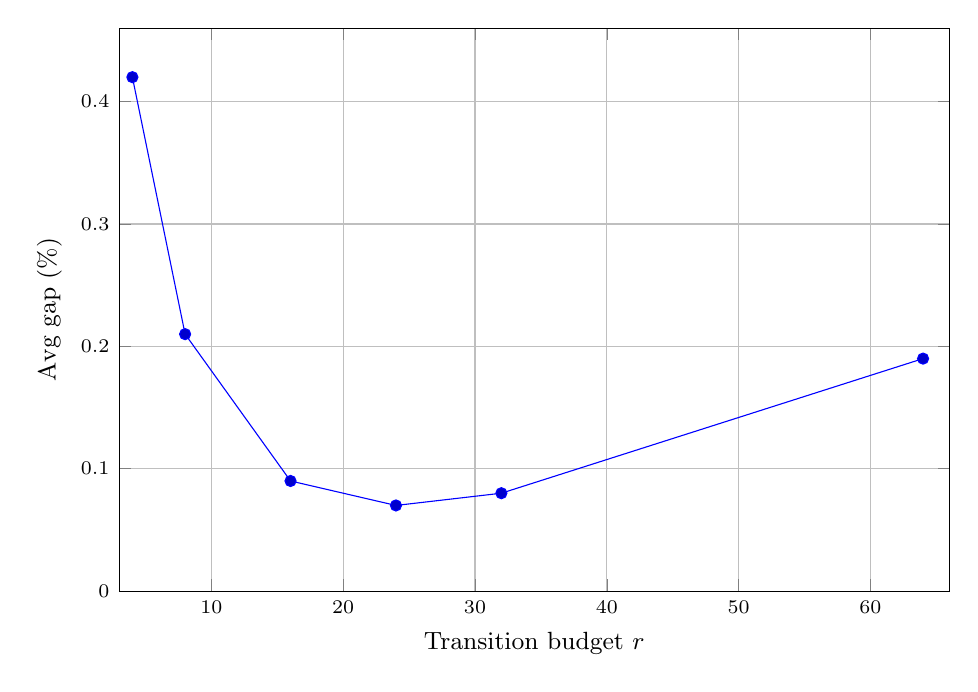
\begin{tikzpicture}
\begin{axis}[
    width=\linewidth,
    height=0.72\linewidth,
    xlabel={Transition budget $r$},
    ylabel={Avg gap (\%)},
    xmin=3, xmax=66,
    ymin=0, ymax=0.46,
    grid=both,
    tick label style={font=\scriptsize},
    label style={font=\small}
]
\addplot+[mark=*] coordinates {(4,0.42) (8,0.21) (16,0.09) (24,0.07) (32,0.08) (64,0.19)};
\end{axis}
\end{tikzpicture}
\end{minipage}
\hfill
\begin{minipage}{0.48\linewidth}
\centering
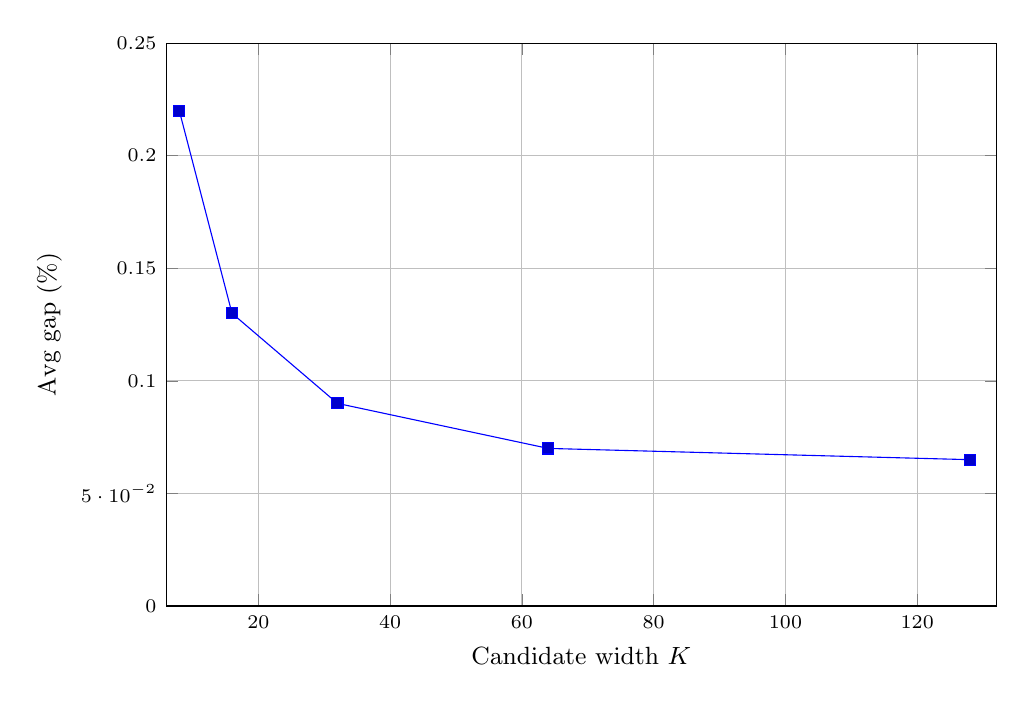
\begin{tikzpicture}
\begin{axis}[
    width=\linewidth,
    height=0.72\linewidth,
    xlabel={Candidate width $K$},
    ylabel={Avg gap (\%)},
    xmin=6, xmax=132,
    ymin=0, ymax=0.25,
    grid=both,
    tick label style={font=\scriptsize},
    label style={font=\small}
]
\addplot+[mark=square*] coordinates {(8,0.22) (16,0.13) (32,0.09) (64,0.07) (128,0.065)};
\end{axis}
\end{tikzpicture}
\end{minipage}
\caption{Sensitivity to transition budget $r$ and projection width $K$ on the small group. The $r$ curve has an intermediate optimum, while the $K$ curve plateaus as the \BTP{} region becomes sufficiently wide.}
\label{fig:sensitivity-rk}
\end{figure}

\subsection{Q6: Does the Interface Transfer Across Policies?}

The plug-and-play evaluation measures architecture dependence by applying the same wrapper across several autoregressive policies without retraining or architecture-specific gradient updates. Table~\ref{tab:policies} reports the resulting gaps.

\begin{table}[t]
\centering
\caption{Plug-and-play behavior across autoregressive policies.}
\label{tab:policies}
\small
\begin{tabularx}{\columnwidth}{lYYYY}
\toprule
\multicolumn{1}{c}{Policy} & \multicolumn{2}{c}{Small group} & \multicolumn{2}{c}{Medium group} \\
\cmidrule(lr){2-3} \cmidrule(lr){4-5}
Policy & Greedy & +\method{} & Greedy & +\method{} \\
\midrule
Attention Model & 11.50\% & 1.08\% & 38.70\% & 6.84\% \\
POMO & 8.74\% & 0.71\% & 32.10\% & 4.35\% \\
\LEHD{} & 4.85\% & 0.18\% & 20.13\% & 3.12\% \\
\SIL{} & 6.07\% & 0.36\% & 9.40\% & 3.42\% \\
\bottomrule
\end{tabularx}
\end{table}

The plug-and-play results indicate that the framework is not tied to a particular architecture. Stronger policies provide better local proposals, but all tested policies benefit from the same scoped test-time loop. The inference interface therefore acts as an independent factor in zero-shot generalization.

\section{Discussion}

The experiments support a simple interpretation: a neural routing policy is most useful when inference preserves the local conditional structure that the policy learned. Full construction makes the neural horizon grow with the route. Broad reconstruction reduces that horizon, but still attaches feedback to a large coupled intervention. \method{} changes the question to a bounded route-conditioned transition, so each call remains local, projectable, and feedback-carrying.

The component results clarify the division of labor. Neural logits provide the learned proposal structure; without them, projection starts from weaker local rearrangements. \BTP{} provides local validation; without it, plausible neural sequences are too rough to compete reliably with a strong reference trajectory. \EAM{} provides stateful reuse; it should not be read as a universal final-gap booster, but as a bounded way to convert positive local advantage into future preferences, especially when route constraints make local outcomes informative.

The main limitation is scope. Very small transition budgets expose only minor local changes, while very large budgets approach broad reconstruction and increase decoding noise and projection cost. Similarly, increasing $K$ improves \BTP{} only until the affected neighborhood is sufficiently covered. The useful regime is therefore intermediate: local enough for dense feedback, but structured enough for the neural model to contribute.

\method{} is not a replacement for classical optimization. LKH-3 and HGS remain strong references. The contribution is to show that autoregressive neural routing can obtain better zero-shot behavior when test-time compute is organized at an appropriate inference granularity. This positions inference-interface design as a complementary axis to architecture and training in neural combinatorial optimization.

\section{Conclusion and Limitations}

We presented \method{}, a training-free inference interface for autoregressive neural routing. The central idea is to change inference granularity: instead of asking a policy to decode a full route or broad reconstruction segment, \method{} asks for bounded route-conditioned transitions, projects them locally, and uses positive local advantage memory to guide future calls. Experiments on representative routing variants show competitive single-route results at much lower runtime than high-budget autoregressive reconstruction, and stronger constrained-routing results than the autoregressive baselines evaluated under the same pipeline. This constrained-routing gain is the clearest evidence for the proposed mechanism: when feasibility and cost depend on route-level interactions, local proposal validation and credit assignment become especially valuable.

The evaluation uses two representative routing variants and a strong autoregressive decoder, with broader scale comparison reported through survey baselines and partial projection-baseline runs reported for the shared benchmark subset. Extending the same protocol requires hardware-controlled runtime measurements and a more detailed accounting of candidate-list construction, neural evaluation, and trajectory projection. Additional architectures, multi-seed variance for stochastic proposal sampling, normalized runtime on shared hardware, and adaptive scope selection are important extensions of the same inference-interface thesis.

\newpage
\appendix

\section{Detailed Component Algorithms}

\begin{algorithm}[h]
\caption{Context-preserving transition.}
\label{alg:cpp}
\small
\begin{algorithmic}[1]
\REQUIRE Reference trajectory $y$, transition budget $r$, start mode
\STATE Select a route position according to the start mode
\STATE Initialize the current anchor and feasible candidate mask
\WHILE{fewer than $r$ new route relations have been introduced}
    \STATE Query the autoregressive policy under the current mask
    \STATE Insert the selected node after the current anchor
    \STATE Update the anchor, route context, and feasible mask
\ENDWHILE
\STATE \textbf{return} candidate route and changed edges
\end{algorithmic}
\end{algorithm}

\begin{algorithm}[h]
\caption{\EAM{} update for one projected proposal.}
\label{alg:eam}
\small
\begin{algorithmic}[1]
\REQUIRE Reference trajectory $y$, candidate trajectory $\hat y$, episodic memory $M$
\STATE Compute advantage $A$ from Eq.~\eqref{eq:advantage}
\IF{$A\le0$}
    \STATE \textbf{return} $M$
\ENDIF
\STATE Compute introduced edges $\Delta E^+$
\FOR{$e\in\Delta E^+$}
    \STATE $M(e)\leftarrow\clip(M(e)+\eta A,-M_{\max},M_{\max})$
\ENDFOR
\STATE \textbf{return} $M$
\end{algorithmic}
\end{algorithm}

\subsection{Trajectory Projection Details}
\label{app:btp-details}

\BTP{} uses a checklist repair procedure adapted to the autoregressive transition setting. The checklist is initialized from the endpoints of edges deleted or inserted by the neural transition. Whenever a projected move is accepted, the endpoints whose incident edges changed are reinserted into the checklist. This mirrors the locality principle of prior bounded correction work \citep{dynaco} while changing the proposal source from ACO perturbations to masked autoregressive transitions.

For \TSP{}, the only projection operator is candidate-graph 2-opt. For a checklist node $u$, \BTP{} scans at most $K$ nearest candidates $v\in\cN_K(u)$ and evaluates segment reversals that replace an incident edge of $u$, either $(u,\operatorname{succ}(u))$ or $(\operatorname{pred}(u),u)$, with a shorter connection to $v$ and the corresponding opposite endpoint. The best positive-gain reversal is applied, and the four affected endpoints are added back to the checklist. Thus the \TSP{} projection reaches a candidate-graph 2-opt fixed point inside the propagated affected region.

For \CVRP{}, \BTP{} first applies the same candidate-graph 2-opt logic within each route. It then scans cross-route candidate pairs touching the checklist and evaluates three capacity-preserving operators: relocating one customer into a neighboring route, swapping two customers across routes, and 2-opt* tail exchange between two routes. A final intra-route 2-opt pass is applied after cross-route changes because inter-route moves can create new within-route inversions. All \CVRP{} moves reject candidates that violate route capacity.

\begin{algorithm}[h]
\caption{\BTP{} for autoregressive transitions.}
\label{alg:btp}
\small
\begin{algorithmic}[1]
\REQUIRE Candidate trajectory $\hat y$, deleted edges $D$, inserted edges $I$, candidate lists $\cN_K$, move cap $h$
\STATE Initialize affected endpoints $A^{\mathrm{end}}$ from $D\cup I$
\STATE Build $\Omega=A^{\mathrm{end}}\cup\bigcup_{i\in A^{\mathrm{end}}}\cN_K(i)$
\STATE Initialize a checklist with nodes in $\Omega$
\WHILE{the checklist is nonempty and fewer than $h$ corrections have been accepted}
    \STATE Pop a checklist node $u$
    \IF{the instance is \TSP{}}
        \STATE Evaluate candidate-graph 2-opt reversals between the incident edges of $u$ and $\cN_K(u)$
    \ELSE
        \STATE Evaluate capacity-feasible intra-route 2-opt, inter-route relocate, swap, and 2-opt* moves touching $u$
    \ENDIF
    \IF{an improving scoped correction exists}
        \STATE Apply the best correction and add newly affected endpoints to the checklist
    \ELSE
        \STATE Mark $u$ as exhausted for the current pass
    \ENDIF
\ENDWHILE
\STATE \textbf{return} $\hat y$
\end{algorithmic}
\end{algorithm}

\section{Extended Baseline Comparison}
\label{app:large-comparison}

Table~\ref{tab:expanded-comparison} reports the broader survey-shaped comparison. It is moved to the appendix to keep the main text focused on the mechanism and the currently evaluated groups, while still showing the wider benchmark context.

\begin{table*}[h]
\centering
\caption{Structured comparison on \TSP{} and \CVRP{} up to 100K nodes. Baseline rows follow the neural routing solver survey \citep{nrs_survey}; each scale group reports average gap, average time, and valid feasible outputs. Heatmap-based rows such as GFACS are excluded because this comparison focuses on autoregressive policies and autoregressive reconstruction/improvement methods.}
\label{tab:expanded-comparison}
\scriptsize
\renewcommand{\arraystretch}{0.82}
\resizebox{\textwidth}{!}{%
\begin{tabular}{@{}lccccccccc@{}}
\toprule
& \multicolumn{3}{c}{Small $(0,1K)$} & \multicolumn{3}{c}{Medium $[1K,10K)$} & \multicolumn{3}{c}{Large $[10K,100K]$} \\
\cmidrule(lr){2-4} \cmidrule(lr){5-7} \cmidrule(lr){8-10}
Method & Gap & Time & Valid & Gap & Time & Valid & Gap & Time & Valid \\
\midrule
LKH-3 & 0.00\% & 7.88s & 69/69 & 0.01\% & 10.52m & 109/109 & 0.08\% & 4.06h & 50/50 \\
\midrule
\SIL{} greedy  & 6.07\% & 1.72s & 69/69 & 9.40\% & 17.87s & 109/109 & 11.11\% & 7.18m & 50/50 \\
BQ & 5.00\% & 2.51s & 68/69 & 19.03\% & 22.74s & 92/109 & 52.00\% & 3.13m & 4/50 \\
\LEHD{} greedy & 4.85\% & 1.01s & 69/69 & 20.13\% & 1.14m & 106/109 & 49.35\% & 23.10m & 11/50 \\
H-TSP  & 6.10\% & 0.61s & 36/69 & 11.62\% & 3.15s & 100/109 & 12.29\% & 21.44s & 40/50 \\
TTPL-MVDF greedy & 3.4759\% & 1.35s & 69/69 & -- & -- & -- & -- & -- & -- \\
\LEHD{} \RRC{}1K & 1.73\% & 8.31m & 69/69 & 10.87\% & 27.24m & 109/109 & 24.02\% & 46.16m & 9/50 \\
\SIL{} \PRC{}1K  & 0.55\% & 14.86m & 69/69 & 2.56\% & 47.99m & 109/109 & 4.55\% & 1.37h & 50/50 \\
DRHG T=1K & \textbf{0.10\%} & 12.83m & 69/69 & \textbf{1.46\%} & 47.63m & 109/109 & \textbf{4.46\%} & 50.07m & 50/50 \\
\method{} & 0.36\% & \textbf{54.02s} & 69/69 & 3.42\% & \textbf{1.43m} & 109/109 & -- & -- & -- \\
\midrule
\midrule
& \multicolumn{3}{c}{Small $(0,1K)$} & \multicolumn{3}{c}{Medium $[1K,10K)$} & \multicolumn{3}{c}{Large $[10K,100K]$} \\
\cmidrule(lr){2-4} \cmidrule(lr){5-7} \cmidrule(lr){8-10}
Method & Gap & Time & Valid & Gap & Time & Valid & Gap & Time & Valid \\
\midrule
\multicolumn{10}{@{}l}{\textbf{\CVRP{}}} \\
\midrule
HGS $t=n/3$ & \textbf{0.29\%} & 1.85m & 99/99 & \textbf{3.59\%} & 23.81m & 5/5 & 7.86\% & 1.92h & 6/6 \\
\midrule
\SIL{} greedy  & 40.04\% & 2.48s & 65/99 & 16.09\% & 26.86s & 5/5 & 10.81\% & 2.45m & 6/6 \\
BQ & 8.87\% & 3.63s & 99/99 & 20.28\% & 39.97s & 5/5 & 41.52\% & 3.38m & 5/6 \\
\LEHD{} greedy & 11.25\% & 1.53s & 98/99 & 19.22\% & 1.66m & 5/5 & 32.80\% & 14.20m & 2/6 \\
TTPL-MVDF greedy & 10.8541\% & 2.34s & 99/99 & -- & -- & -- & -- & -- & -- \\
\LEHD{} \RRC{}1K & 3.58\% & 13.27m & 99/99 & 11.73\% & 34.06m & 5/5 & 21.98\% & 47.00m & 2/6 \\
TTPL-MVDF \RRC{}100 & 5.9292\% & 31.07s & 99/99 & -- & -- & -- & -- & -- & -- \\
\SIL{} \PRC{}1K  & 21.38\% & 21.80m & 99/99 & 8.28\% & 57.86m & 5/5 & \textbf{7.40\%} & 1.18h & 6/6 \\
DRHG T=1K & 11.11\% & 18.58m & 99/99 & 17.95\% & 42.15m & 5/5 & 16.95\% & 1.49h & 6/6 \\
\method{} & \textbf{2.47\%} & \textbf{2.23m} & 99/99 & \textbf{4.76\%} & \textbf{14.76m} & 5/5 & 7.64\% & \textbf{44.21m} & 6/6 \\
\bottomrule
\end{tabular}%
}
\end{table*}

\section{Additional Experimental Details}

\paragraph{Evaluation protocol.}
We use the benchmark pool and scale grouping defined by the neural routing solver survey \citep{nrs_survey}. The test pool consists of established benchmark and challenge instances with available best-known solutions: TSPLIB \citep{tsplib}, National TSP, VLSI, and DIMACS challenge instances \citep{national_tsp,vlsi_tsp,dimacs_tsp} for the single-route benchmark, and CVRPLIB \citep{cvrplib} for capacitated routing. Results are grouped into small $(0,1K)$, medium $[1K,10K)$, and large $[10K,100K]$ buckets. Each run starts from an initial feasible route, performs a fixed number of outer iterations, and returns the best route found. A run is counted as valid when it returns a feasible route with finite cost.

The comparison follows the survey pipeline's emphasis on three complementary axes: effectiveness, measured by optimality gap to the best known solution; efficiency, measured by runtime; and reliability, measured by valid feasible coverage. Runtime is reported when available; our method and the projection baseline use the same local hardware environment for the completed local runs.

\begin{table}[h]
\centering
\caption{Main configurations used for the evaluated benchmark groups.}
\small
\begin{tabularx}{\columnwidth}{lYY}
\toprule
Parameter & Small & Medium \\
\midrule
\multicolumn{3}{l}{\textbf{Policy and problem scope}} \\
Default logit provider & \multicolumn{2}{c}{\SIL{} autoregressive decoder \citep{sil}} \\
Problems & \TSP{}, \CVRP{} & \TSP{}, \CVRP{} \\
\midrule
\multicolumn{3}{l}{\textbf{Inference budget}} \\
Outer iterations & 100 & 100 \\
Neural proposals per iteration & 100 & 100 \\
Minimum new-edge threshold & 24 & 8 \\
\midrule
\multicolumn{3}{l}{\textbf{State and update rules}} \\
Start mode & \multicolumn{2}{c}{default random route anchor} \\
Memory update & \multicolumn{2}{c}{\EAM{} introduced-edge credit} \\
Reference update & \multicolumn{2}{c}{Best projected proposal with monotone best-so-far output} \\
Neural weight updates & \multicolumn{2}{c}{None} \\
\bottomrule
\end{tabularx}
\end{table}

\paragraph{Neural logit provider.}
The main experiments use the Self-Improved Learning autoregressive decoder \citep{sil} under local masked states. We do not modify its architecture, training objective, or learned parameters. This isolates the effect of the inference interface from the effect of retraining or redesigning the neural model.

\paragraph{Configuration selection.}
The 15-instance validation study indicates that wider transition and projection neighborhoods improve solution quality on small held-out instances. The strongest validation configuration uses random start mode, introduced-edge advantage memory, transition budget 24, and projection width 64. The full sensitivity experiments in the main text report the all-instance structure used for the main results.

\begin{table}[h]
\centering
\caption{Validation ablation on 15 held-out small \TSP{} instances.}
\label{tab:validation-small}
\small
\begin{tabularx}{\columnwidth}{lYYYYYY}
\toprule
\multicolumn{4}{c}{Configuration} & \multicolumn{3}{c}{Validation outcome} \\
\cmidrule(lr){1-4} \cmidrule(lr){5-7}
Start & Memory & $r$ & $K$ & Avg gap & Optimal & Avg time \\
\midrule
Hybrid & Source-advantage & 16 & 32 & 0.3039\% & 9/15 & 26.58s \\
Random & None & 16 & 32 & 0.1096\% & 10/15 & 23.01s \\
Random & Source-route & 16 & 32 & 0.1943\% & 6/15 & 27.87s \\
Random & \EAM{} & 16 & 32 & 0.0908\% & 11/15 & 24.01s \\
Random & \EAM{} & 24 & 32 & 0.0335\% & 13/15 & 27.06s \\
Random & \EAM{} & 24 & 64 & \textbf{0.0278\%} & \textbf{14/15} & 27.31s \\
\bottomrule
\end{tabularx}
\end{table}

\section{Per-Instance Extremes}

\begin{table}[h]
\centering
\caption{Best and worst small instances.}
\small
\begin{tabularx}{\columnwidth}{lYY@{\qquad}lYY}
\toprule
\multicolumn{3}{c}{Best cases} & \multicolumn{3}{c}{Worst cases} \\
\cmidrule(lr){1-3} \cmidrule(lr){4-6}
Instance & Gap & Time & Instance & Gap & Time \\
\midrule
wi29 & 0.00\% & 10.33s & p654 & 1.40\% & 35.31s \\
dj38 & 0.00\% & 13.99s & pr439 & 0.62\% & 48.27s \\
eil51 & 0.00\% & 17.98s & pbd984 & 0.48\% & 42.17s \\
berlin52 & 0.00\% & 18.77s & dkg813 & 0.42\% & 44.48s \\
bier127 & 0.00\% & 23.78s & rbu737 & 0.39\% & 36.23s \\
\bottomrule
\end{tabularx}
\end{table}

\begin{table}[h]
\centering
\caption{Best and worst medium instances.}
\small
\begin{tabularx}{\columnwidth}{lYY@{\qquad}lYY}
\toprule
\multicolumn{3}{c}{Best cases} & \multicolumn{3}{c}{Worst cases} \\
\cmidrule(lr){1-3} \cmidrule(lr){4-6}
Instance & Gap & Time & Instance & Gap & Time \\
\midrule
portcgen-1000-10008 & 0.20\% & 48.88s & ja9847 & 4.20\% & 2.88m \\
d1291 & 0.31\% & 1.49m & gr9882 & 3.95\% & 3.09m \\
portcgen-1000-10004 & 0.42\% & 51.91s & ei8246 & 3.71\% & 2.43m \\
portcgen-1000-1000 & 0.48\% & 51.05s & kz9976 & 3.46\% & 3.30m \\
d2103 & 0.52\% & 1.94m & ar9152 & 3.40\% & 3.13m \\
\bottomrule
\end{tabularx}
\end{table}

\section{Diagnostics and Compatibility}

\paragraph{Masked local decoding.}
The method depends on querying the declared neural policy under a local mask. When the model cannot yield logits for a masked state, the corresponding proposal is unsupported and should not be replaced by a non-neural fallback. This convention preserves a clear evaluation of the neural proposal mechanism and avoids conflating learned local transitions with handcrafted proposal rules.

\paragraph{Transition reach.}
When the transition budget is too small, repeated local proposals may tie the reference trajectory without escaping the current basin. Increasing the transition budget expands the reachable transition set, but also broadens the policy query and increases decoding difficulty. The sensitivity study therefore varies both $r$ and $K$.

\paragraph{Memory saturation.}
The clipping rule prevents unbounded memory growth, but saturation can still reduce adaptivity if many edges reach the clipping threshold early. If most nonzero entries saturate, the memory strength $\lambda$, step size $\eta$, or clipping threshold $M_{\max}$ should be reduced.

\paragraph{Projection locality.}
\BTP{} assumes that most damage from a bounded neural transition is near the deleted or inserted edges. If this assumption fails, the projection region may miss improvements that a global correction pass would find. The candidate width $K$ controls this tradeoff: larger values expand the projection neighborhood but increase the number of local evaluations.

\paragraph{Compatibility requirements.}
Applying the framework to an autoregressive policy requires four implementation properties:
\begin{itemize}[leftmargin=*,noitemsep]
  \item \textbf{Masked local logits:} the model must expose a proposal distribution over a bounded feasible set.
  \item \textbf{Stable route context:} the model state must contain enough information to interpret route anchors and candidate nodes.
  \item \textbf{Feasible route transition:} the decoded local sequence must be applicable to the reference trajectory.
  \item \textbf{Problem-aware projection:} the projection step must preserve the constraints of the routing problem.
\end{itemize}
These requirements are mild for autoregressive \TSP{} construction models with explicit masks, but they become more restrictive for constrained routing variants or architectures that do not expose local logits.

\section{Design Rationale}

Constructive neural solvers learn a mapping from partial routing states to next-node decisions. Their main advantage is fast inference once a model has been trained. However, ordinary construction is irreversible: an early poor edge changes the future feasible set and forces later decisions to compensate. Beam search and sampling mitigate this issue by maintaining multiple trajectories, but they still use the model as a trajectory generator. The proposed framework retains the constructive decoder while changing its role. The model repeatedly evaluates small route-conditioned transition states, while the reference trajectory supplies context and the outer inference loop supplies feedback.

This design is related to reconstruction-style inference, which modifies part of a solution and queries a policy to complete the missing structure. Both approaches improve a reference trajectory through local intervention, but STAR uses a bounded route transition rather than a broad reconstruction. Large transitions increase decoding noise and projection cost, while very small transitions approach deterministic local correction. The method therefore operates in an intermediate regime in which the transition is local enough for immediate projection but structured enough for the neural model to contribute learned conditional information.

The memory representation also reflects this training-free guidance view. Actions are state-dependent: the same node choice can represent different structural changes depending on the current anchor and mask. Edges provide a more stable representation of route structure. \EAM{} therefore stores edge credit and maps it back to action scores through $\phi(s,a)$. This creates a lightweight memory that is independent of the internal parameterization of the neural policy.

Positive credit and monotone best-so-far tracking provide a conservative anytime output. Negative credit is tempting, but the signal from a failed proposal is ambiguous. A proposal may fail because the local context was poorly chosen, the neural sequence was weak, projection was too narrow, or the reference trajectory was already locally strong. Positive improvements provide clearer evidence: they identify transitions that survived projection and reduced cost. The reference trajectory can still move to the best projected proposal for exploration, while the returned best-so-far solution remains monotone.

\section{Extension to Capacitated Routing}

For \CVRP{}, we use a capacity-aware local state and projection operator. The local state includes depot position, route boundaries, customer demands, and remaining route capacity. The decoder mask prevents infeasible insertions. The projection step uses capacity-preserving local corrections. These requirements preserve the conceptual framework while adapting the feasibility machinery to capacitated routing.

\bibliographystyle{plainnat}
\bibliography{references}

\end{document}
